\documentclass{article}
\usepackage{graphicx}
\usepackage{amsmath}
\usepackage{subcaption}
\begin{document}
\tableofcontents
\listoffigures
\section{Section}

Hello World!

\subsection{Math Functions in Latex}
There are two major modes of typesetting math in LaTeX one is
 embedding the math directly into your text by encapsulating your 
 formula in dollar \$ signs and the other
 is using a predefined math environment.


\begin{equation*}
  f(x) = x^2
\end{equation*}

\subsubsection{Subsubsection}


% Using inline math – embed formulas in your text

% To make use of the inline math feature, simply write your text and 
% if you need to typeset a single math symbol or formula, surround it with dollar signs:
% ...
This formula $f(x) = x^2$ is an example.


% The most useful math envorinments are the equation environment for 
% typesetting single equations and the align environment for 
% multiple equations and automatic alignment:

\begin{equation*}
    1 + 2 = 3 
  \end{equation*}
  \begin{equation*}
    1 = 3 - 2 
    % \\
    % x = y + 3
  \end{equation*}
  \begin{align*}
    1 + 2 &= 3\\
    1 &= 3 - 2
  \end{align*}


\paragraph{Fractions and More}
LaTeX is capable of displaying any mathematical notation. 
It’s possible to typeset integrals, fractions and more. 
Every command has a specific syntax to use. 
\begin{align*}
    f(x) &= x^2\\
    g(x) &= \frac{1}{x}\\
    F(x) &= \int^a_b \frac{1}{3}x^3
  \end{align*}

 
It is also possible to combine various 
commands to create more sophisticated expressions such as:

\begin{align*}
    \frac{1}{\sqrt{x}}
  \end{align*}

\subsection{Matrices}
\begin{align*}
\begin{matrix}
    1 & 0\\
    0 & 1
\end{matrix}
\end{align*}


% To surround the matrix by brackets, 
% it’s necessary to use special statements, 
% because the plain [ ] symbols do not scale as the matrix grows. 
% The following code will result in wrong brackets:

\begin{align*}
[
    \begin{matrix}
1 & 0\\
0 & 1
\end{matrix}
]
\end{align*}



\begin{align*}
    \left[
        \begin{matrix}
    1 & 0\\
    0 & 1
    \end{matrix}
    \right]
    \end{align*}
\section{Figures and Images in {\sc Latex}}


\begin{itemize}
    \item Captioned images / figures in LaTeX
    \item Image positioning / setting the float
    \item Multiple images / subfigures in LaTeX

\end{itemize}
\subsection{Captioned images / figures in LaTeX}

\begin{figure}[h!]
    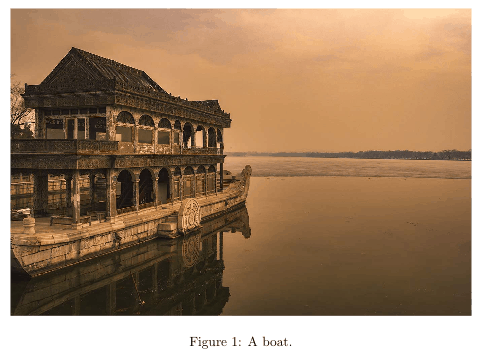
\includegraphics[width=0.5\textwidth]{boat.png}
    \caption{A boat.}
    \label{fig:boat1}
  \end{figure}
  

  \subsection{Multiple Images}
%...

\begin{figure}[h!]
    \centering
    \begin{subfigure}[b]{0.4\linewidth}
      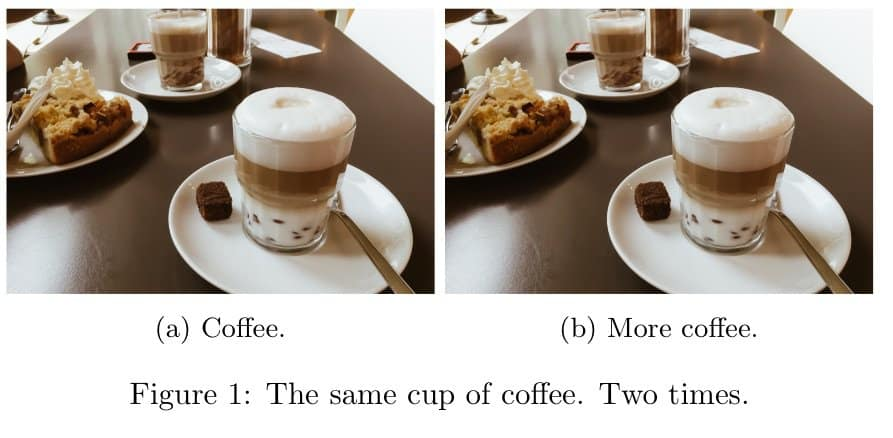
\includegraphics[width=\linewidth]{coffee.jpg}
      \caption{Coffee.}
    \end{subfigure}
    \begin{subfigure}[b]{0.4\linewidth}
      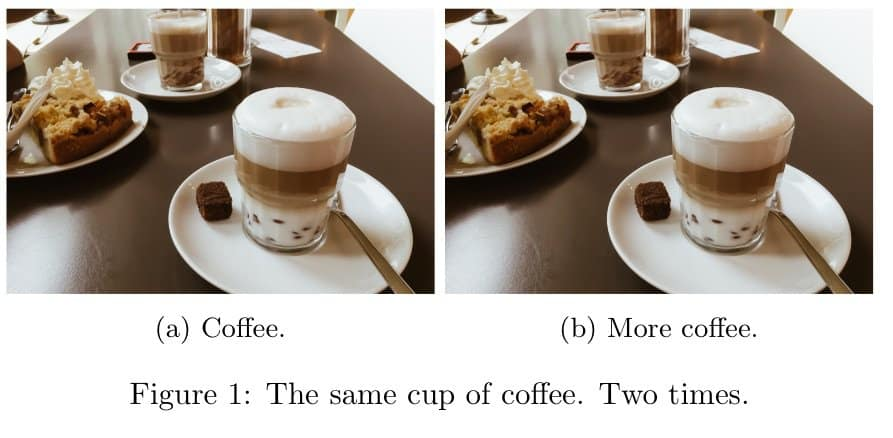
\includegraphics[width=\linewidth]{coffee.jpg}
      \caption{More coffee.}
    \end{subfigure}
    \caption{The same cup of coffee. Two times.}
    \label{fig:coffee}
  \end{figure}
  
  %...
  \section{Biblio}
  Random citation~\cite{DUMMY:1} embeddeed in text.
  Donald Knuth~\cite{don}


  \bibliography{sdf} 
  \bibliographystyle{ieeetr}
\end{document}

